\documentclass[]{article}

% Packages/Macros
\usepackage{amssymb}
\usepackage{latexsym}
\usepackage{amsmath}
\usepackage{graphicx}
\usepackage{fixltx2e}
\usepackage[letterpaper,left=1in,right=1in,top=0.8in,bottom=0.8in,footskip=0.25in]{geometry}
\usepackage{color}
\usepackage{subcaption}
\usepackage{float}

% Document
\begin{document}

\title{\vspace{-15mm}CS 6505 Bloom Filters Project Report}
\author{Pavel Komarov}
\maketitle
  
  
  \section{Introduction}
  \vspace{-2mm}
  Bloom filters keep an array $H$ of $n$ bits initially set to 0. Insertion is done by hashing an input $x$ $k$ times with $k$ different hash functions and setting the corresponding $k$ bits in $H$ to 1. Querying is done by hashing a value $y$ $k$ times with the same $k$ hash functions used for insertion and checking to see whether all $k$ of those bits are 1. The brilliance of this approach is that both insertion and querying can be done in $O(1)$ with very, very little space, efficiencies traditional hash tables can not reach. The trouble, of course, is that there is some nonzero probability that all $k$ bits accessed in a query were set to 1 by additions of $x$s that were not $y$. The purpose of this project is to do some analysis of that error rate.
  \vspace{-3mm}

  \section{Hashing Machinery: A Foray in to Probability}
  \vspace{-2mm}
  Early on I got stuck wondering how I could hash numbers simply for insertion and then reproduce those same hashes at query-time. Ideally, I would have $k$ functions that all output perfectly uniform distributions given any inputs, but implementing such functions is potentially very complicated. To find a solution, I created Analysis.java and Analysis.m and tried several mathematical manipulations based on multiplication and overflow. The results were random in some cases but not for all cases. Eventually I realized a random number XOR a random number is a random number, so I could keep a vector of $k$ random numbers and XOR with inputs to simulate a call to hash(input). 
  
  To prove the validity of this approach, I ran simulations. For two simulated hashes, \textbf{Figure 1} depicts the contents of $n = 1000$ ``bins'' filled with $m = 1000000$ ``balls'' ((a) and (c)) as well as histograms of the number of bins that contain $b\pm q$ balls ((b) and (d)). For all simulated hashes I have tried (dozens), the results look like this white noise.

  \vspace{-2mm}
  \begin{figure}[H]
    \centering
    \begin{subfigure}{.235\textwidth}
      \centering
      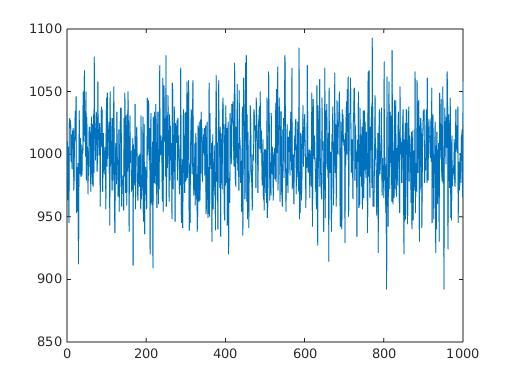
\includegraphics[width=1\linewidth]{noise1.jpg}
      \vspace{-6mm}
      \caption{}
    \end{subfigure}
    \begin{subfigure}{.235\textwidth}
      \centering
      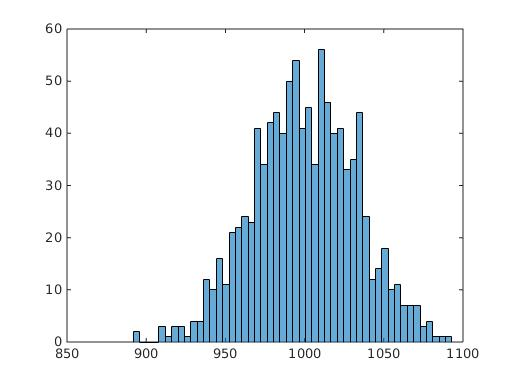
\includegraphics[width=1\linewidth]{noisehist1.jpg}
      \vspace{-6mm}
      \caption{}
    \end{subfigure}
    \begin{subfigure}{.235\textwidth}
      \centering
      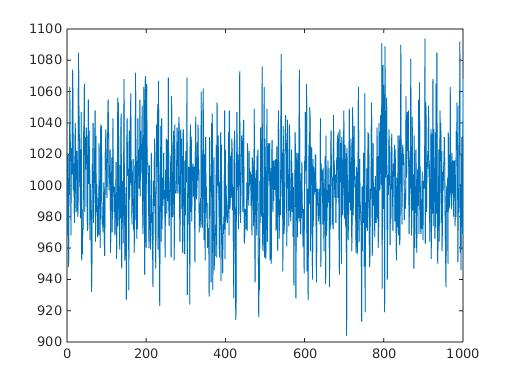
\includegraphics[width=1\linewidth]{noise2.jpg}
      \vspace{-6mm}
      \caption{}
    \end{subfigure}
    \begin{subfigure}{.235\textwidth}
      \centering
      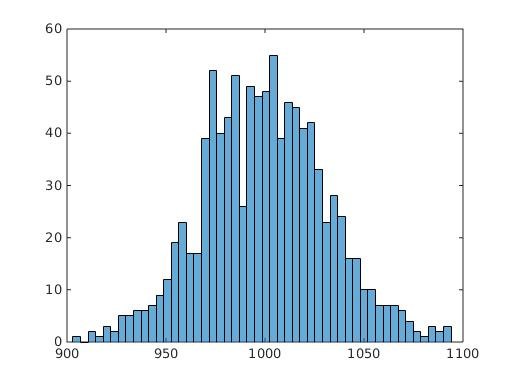
\includegraphics[width=1\linewidth]{noisehist2.jpg}
      \vspace{-6mm}
      \caption{}
    \end{subfigure}
    \vspace{-2mm}
    \caption{Analysis of simulated hash function demonstrating that input XOR $k$th random number is valid.}
  \end{figure}

  \vspace{-3mm}
  To make further sense of the above, recall that the probability a given bin $i$ in $H$ holds $b$ balls is given by Bernoulli trials as:
  \vspace{-5mm}

  $$Pr[H_{i} = b] = {m \choose b}\left(\frac{1}{n}\right)^{b}\left(1 - \frac{1}{n}\right)^{m-b}$$

  \noindent
  By the central limit theorem, as the number of trials goes to infinity, the distribution of these new random variables is given by a Gaussian iff the underlying trials are independent, which is as I observe. So, since these hash-events are independent, and since the mean of the output is centered around $E[balls\ per\ bin] = \frac{m}{n}$, this method of simulating hashes does exactly what a real hash function would do.
  \vspace{-4mm}

  \section{Theory: The Math}
  \vspace{-2mm}
  First, a derivation of the theoretical error rate for Bloom Filters. This math is important to fully understand the results given hereafter.
  \vspace{-1mm}
  $$Pr(false\ positive|input\ y) = Pr(H[h_{1}(y)] = 1\ \wedge\ H[h_{2}(y)] = 1\ \wedge ... H[h_{k}(y)] = 1),\ where\ h_{x}\ is\ a\ hash\ function$$
  \vspace{-6mm}
  $$hashes\ are\ indep. \implies above = Pr(H[h_{1}(y)] = 1)\ \wedge\ Pr(H[h_{2}(y)] = 1)\ \wedge ... Pr(H[h_{k}(y)] = 1) = Pr(H[bit] = 1)^{k}$$
  $$Pr(H[bit] = 1) = 1 - Pr(H[bit] = 0),\ Pr(H[bit] = 0 | 1\ trial) = (1 - 1/n)$$
  $$|insertions|\cdot|hash functions| = mk\ trials \rightarrow Pr(H[bit] = 0 | mk\ trials) = (1 - 1/n)^{mk}$$
  $$\implies Pr(false\ positive|y,\ m\ insertions) = (1 - (1 - 1/n)^{mk}))^{k}$$ 
  $$But:\ (1 - 1/n) \approx e^{-1/n}\ for\ large\ n,\ and\ \lim_{n\to\infty} (1 - 1/n) = \lim_{n\to\infty} e^{-1/n} = 1,\ so:$$
  \vspace{-4mm}
  $$Pr(false\ positive|y,\ m\ insertions) \approx (1 - e^{-mk/n})^{k}\ (= as\ n \rightarrow \infty)$$
  \vspace{-9mm}

  \section{Simulation and Results}
  \vspace{-2mm}
  My BloomFilter.java code implements the insert and query functionality described in the intro backed by an array of $\lceil\frac{n}{32}\rceil$ ints and utilizing the simulated hashes described in \textbf{Section 2}. I use $k = \frac{n}{m}ln(2)$ (or the nearest integer) hash functions, the number which minimizes false positives, as found from the critical point of $(1 - e^{-mk/n})^{k}$. See my code for all the details; it's fairly straight-forward.

  The simulation itself works by iterating over $n \in \{10, 10^{2}, 10^{3}, 10^{4}, 10^{5}, 10^{6}\}$ and $c = \frac{n}{m} \in \{1, 2, 5, 10, 25, 100\}$ (which all divide $n$ evenly). On each pass I set up the Bloom Filter anew for that $(n,c)$, insert $m$ random numbers, query over [0,max int-1] (my chosen universe) to find all ``true'' responses, calculate the false-positive rate with
  $$rate_{FP} = \frac{|FP|}{|FP|+|TN|} = \frac{|P|-|TP|}{|Universe|-|TP|},$$
  and finally write results to a file. I force a repeat trial for each $(n,c)$ pair five times so I can see variance.

  After a couple of hours for run-time, I processed the results in Matlab with BloomFilter.m to generate the plots shown in \textbf{Figure 2}. Since $rate_{FP} \rightarrow 0$ as $c\ \rightarrow \infty$, I have shown the data on a log-log scale in addition to log-linear.
  
  \vspace{-4mm}
  \begin{figure}[H]
    \centering
    \begin{subfigure}{.49\textwidth}
      \centering
      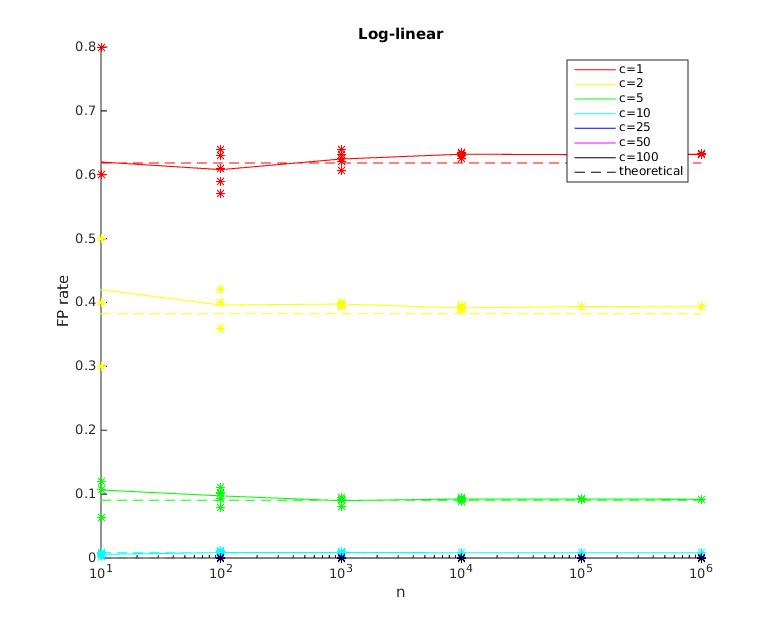
\includegraphics[width=1\linewidth]{loglinear.jpg}
      \vspace{-9mm}
      \caption{}
    \end{subfigure}
    \begin{subfigure}{.49\textwidth}
      \centering
      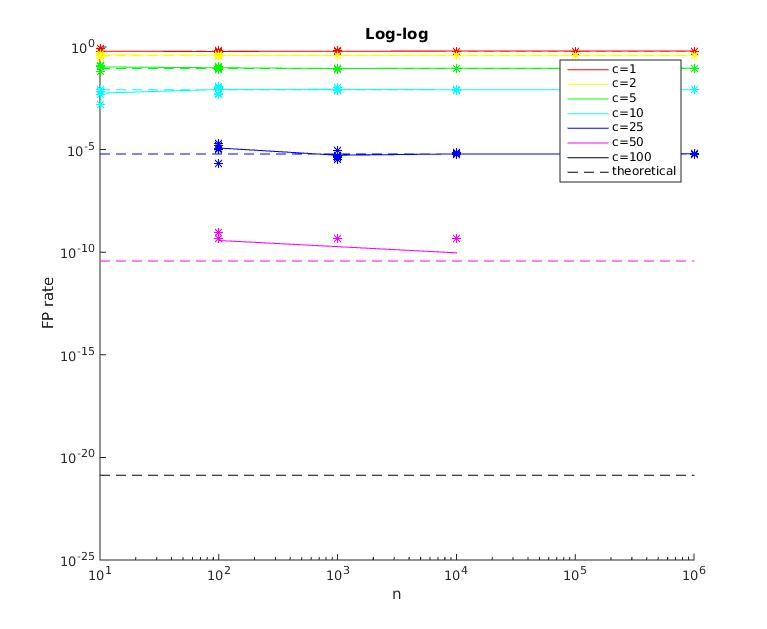
\includegraphics[width=1\linewidth]{loglog.jpg}
      \vspace{-9mm}
      \caption{}
    \end{subfigure}
    \vspace{-2mm}
    \caption{Bloom Filter false positive rates for multiple values of c as n increases.}
  \end{figure}

  \vspace{-4mm}
  One should notice immediately that increasing $c$ does wonders for the error rate. At c = 50, I only observe a false positive on a small fraction of my trials, and at c = 100, I observe none. The reason for this should be clear: My universe is $2^{31}-1$ elements large, and the theoretical error rate for this $c$ is $\frac{1}{2}^{100ln(2)}$. The product of these numbers, the probability I see a false positive on any given run, is $2.92 \cdot 10^{-12}$!

  The other important result from this analysis is less obvious but just as important. Notice there is more variation between datapoints at small $n$, but as $n$ grows this variance shrinks, and trials fit more tightly to the theoretical prediction. The reason for this is in the math: Remember the functions $(1-1/n)$ and $e^{-1/n}$ are better approximations of each other as $n \rightarrow \infty$.
  \vspace{-4mm}

  \section{Conclusion}
  \vspace{-2mm}
  This class is the first place I have ever heard of Bloom Filters. Considering how fast they are, how little space they take, and how low their error rates can be, I will keep them in mind for applications where a very few false-positives is okay.

  I am including all of the files I used to generate this report in my submission, probably more than you want. Focus on BloomFilter.java if you only have time for one.

\end{document}
